\documentclass[14pt]{extarticle}

\usepackage{fontspec}
\setmainfont{Times New Roman}

% размер полей
\usepackage{geometry}
\geometry{a4paper, top=2cm, bottom=2cm, right=1.5cm, left=3cm}

 %debugging
%\usepackage{showframe}

% полуторный интервал
\usepackage{setspace}
\onehalfspacing

% абзацный отступ
\setlength{\parindent}{1.25cm}

% выравнивание текста по ширине
\sloppy

% списки
\usepackage{calc} % арифметические операции с величинами
\usepackage{enumitem}
\setlist{
    nosep,
    leftmargin=0pt,
    itemindent=\parindent + \labelwidth - \labelsep,
}

% подписи к рисункам и таблицам
\usepackage{caption}
\renewcommand{\figurename}{Рисунок}
\renewcommand{\tablename}{Таблица}
\DeclareCaptionFormat{custom}
{
    \textit{#1#2#3}
}
\DeclareCaptionLabelSeparator{custom}{. }
\captionsetup{
    % хз какой это размер - 12 или нет, но выглядит меньше 14
    font=small,
    format=custom,
    labelsep=custom,
}

% картинки
\usepackage{graphicx}

% колонтитулы
\usepackage{fancyhdr}

% картинки и таблицы находятся именно в том месте текста где помещены (атрибут H)
\usepackage{float}

% таблицы
\usepackage{tabularray}

\graphicspath{ {6.3.4/models/} }
\begin{document}
\pagestyle{fancy}
\fancyhead{}
% disable header
\renewcommand{\headrulewidth}{0pt}
\fancyfoot[L]{Дубровских гр 221-361}
\fancyfoot[C]{ЛР 6.3.4}
\fancyfoot[R]{Продажа автотранспорта}
\singlespacing

\newpage
\begin{center}
    Министерство науки и высшего образования Российской Федерации
    Федеральное государственное автономное образовательное учреждение

    высшего образования

    \guillemotleft МОСКОВСКИЙ ПОЛИТЕХНИЧЕСКИЙ УНИВЕРСИТЕТ\guillemotright

    (МОСКОВСКИЙ ПОЛИТЕХ)
\end{center}
\noindent
\bigbreak
\bigbreak
\bigbreak
\bigbreak
\begin{center}
    ЛАБОРАТОРНАЯ РАБОТА 6.3.4

    По курсу Проектирования пользовательских интерфейсов в веб

    \textbf{Изучение критериев и принципов подбора графического контента для веб}
    \bigbreak
    \bigbreak
    \bigbreak
    \bigbreak
    ТЕМА

    \guillemotleft\textbf{САЙТ ДЛЯ ПРОДАЖИ И ПОИСКА АВТОМОБИЛЕЙ}\guillemotright
\end{center}
\noindent
\bigbreak
\bigbreak
\bigbreak
\bigbreak
\bigbreak
\bigbreak
\bigbreak
\bigbreak
\bigbreak
\bigbreak
\hfill Выполнил

\hfill Дубровских Никита Евгеньевич

\hfill Группа 221-361
\bigbreak
\bigbreak
\bigbreak
\hfill Проверил

\hfill Натур ВВ
\vfill
\begin{center}
    Москва, 2024
\end{center}
\newpage
\onehalfspacing


\begin{center}
    \textbf{Лабораторная работа 6.3.4}

    \textbf{Изучение критериев и принципов подбора графического контента для веб}
\end{center}

\textbf{Цель работы:} подобрать  и подготовить необходимый графический веб-контент пользовательского интерфейса
\bigskip

\textbf{Задачи:}

\begin{enumerate}
    \item Провести анализ скорости загрузки страницы всех сайтов-аналогов на предмет графического контента. Рассмотреть рекомендации по оптимизации изображений анализируемых сайтов и записать в таблицу.
    \item Изучить критерии и принципы подбора графического контента для веб
    \item Подобрать и подготовить изображения в соответствии с тематикой, палитрой, стилем сайта (мобильного приложения) 
    \item Проверить подобранный контент на уникальность. Указать в Сводной таблице
    \item Расположить подобранный графический контент в вайрфреймы и получить макеты.
\end{enumerate}
\bigskip

\textbf{Основные термины}

\begin{itemize}
    \item Графический контент - визуальные элементы, используемые на веб-сайте (изображения, видео, анимация).
    \item Веб-интерфейс - интерфейс, с которым взаимодействует пользователь через веб-браузер.
    \item Оптимизация изображений - процесс уменьшения размера файлов изображений без потери качества для улучшения скорости загрузки страниц.
    \item Вайрфреймы - каркасные макеты, отображающие структуру веб-страницы или приложения.
    \item Скорость загрузки страницы - время, необходимое для полной загрузки веб-страницы, важный фактор пользовательского опыта.
    \item Уникальность контента - оригинальность изображений и других визуальных элементов, важная для SEO и авторских прав.
    \item Атрибут alt - текстовое описание изображения, используемое для доступности и SEO.
    \item Форматы изображений - различные типы файлов, используемых для хранения изображений, такие как JPEG, PNG, GIF, SVG, WEBP.
    \item Эмоциональность изображений - способность изображений вызывать чувства и ассоциации у пользователей.
    \item Стиль и палитра - визуальные характеристики, определяющие внешний вид графического контента в соответствии с темой сайта или приложения.
    \item Типы изображений - классификация визуального контента, включая фотографии, векторную графику, логотипы и иконки.
    \item Инструменты для подбора изображений - сервисы и платформы, помогающие находить графический контент (например, Shutterstock, Multicolr Tineye).
    \item Критерии подбора изображений - основные принципы выбора подходящих изображений для веб-контента.
\end{itemize}
\bigskip

\textbf{auto.ru}
\bigskip

\noindent
\begin{minipage}{\linewidth}
    \fbox{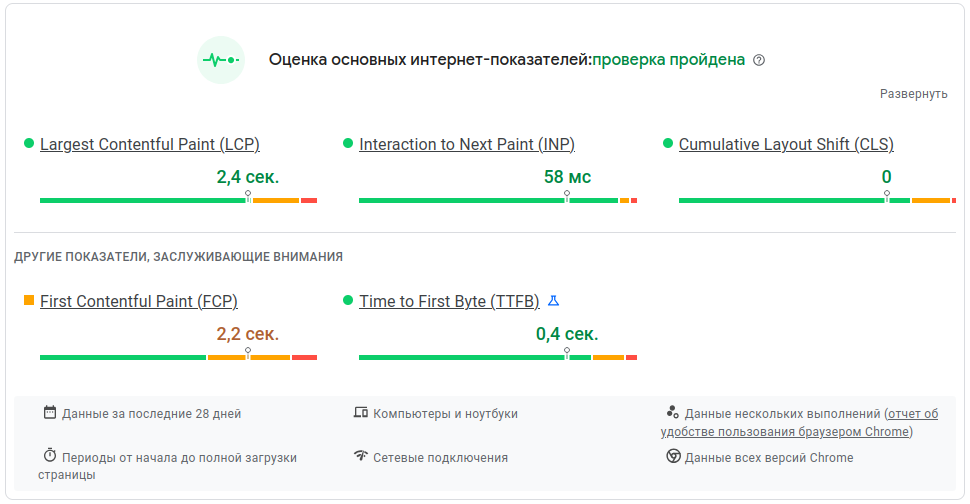
\includegraphics[width=\linewidth]{auto_diag1}}
\end{minipage}
\bigskip

\noindent
\begin{minipage}{\linewidth}
    \fbox{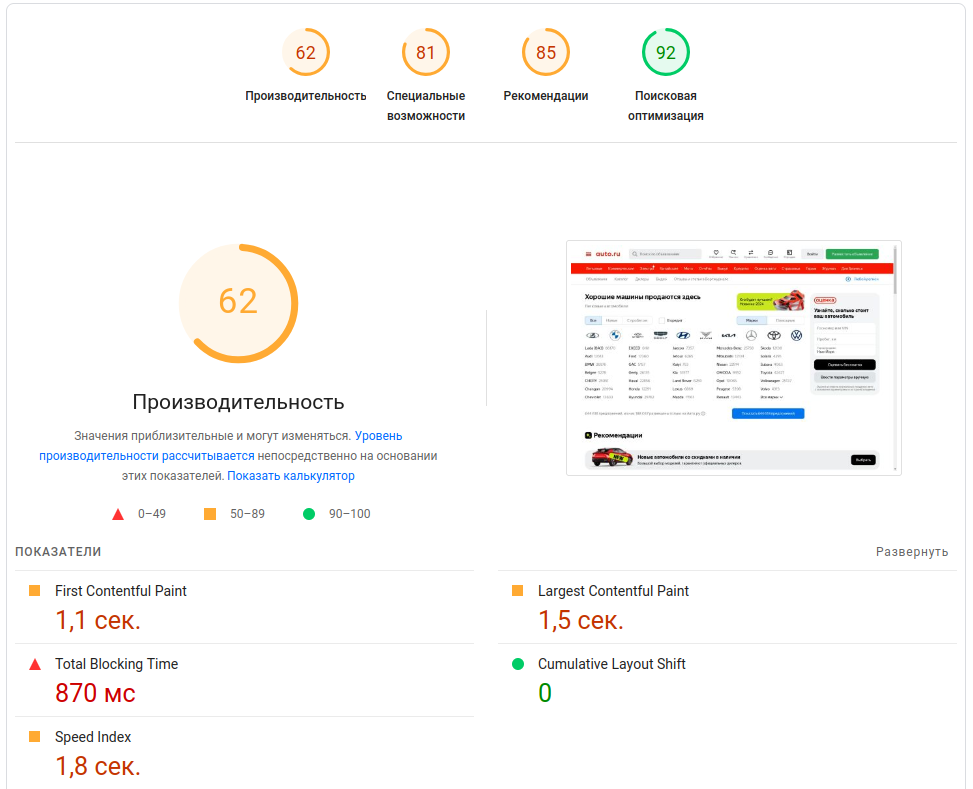
\includegraphics[width=\linewidth]{auto_diag2}}
\end{minipage}
\bigskip

\noindent
\begin{minipage}{\linewidth}
    \fbox{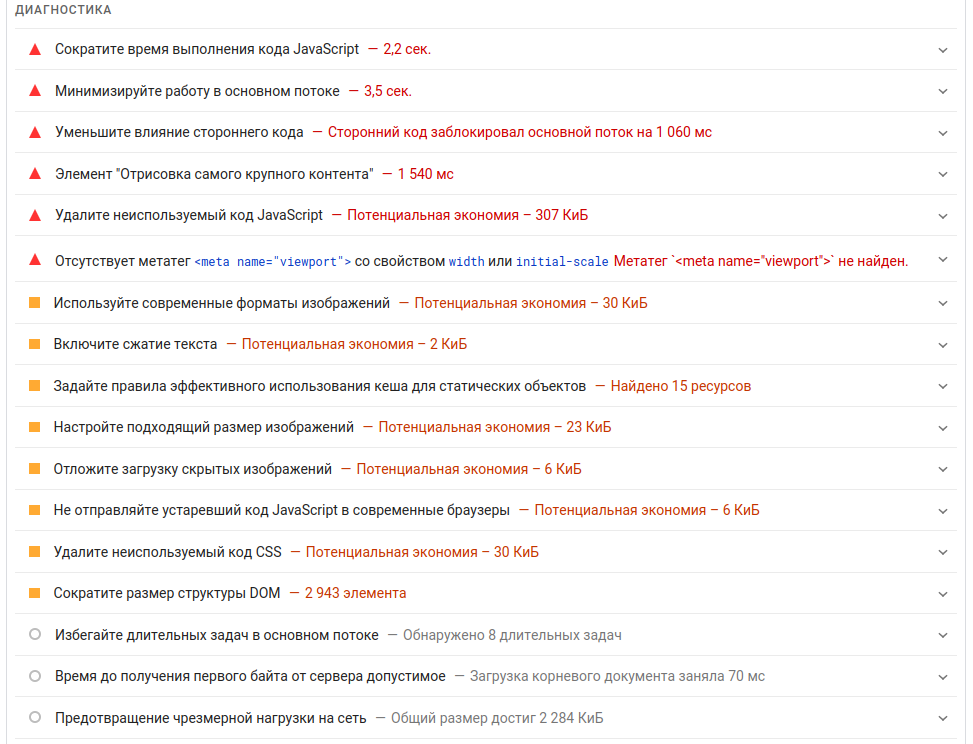
\includegraphics[width=\linewidth]{auto_diag3}}
\end{minipage}
\bigskip

На сайте присутствуют изображения неподходящего размера, и в несовременных форматах. Суммарная потенциальная экономия - 48 КиБ.

\textbf{drom.ru}
\bigskip

\noindent
\begin{minipage}{\linewidth}
    \fbox{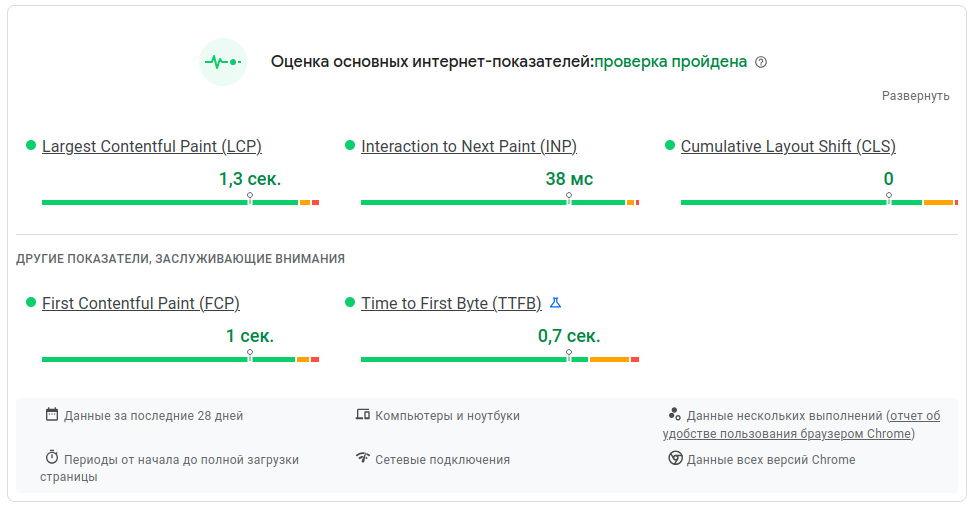
\includegraphics[width=\linewidth]{drom_diag1}}
\end{minipage}
\bigskip

\noindent
\begin{minipage}{\linewidth}
    \fbox{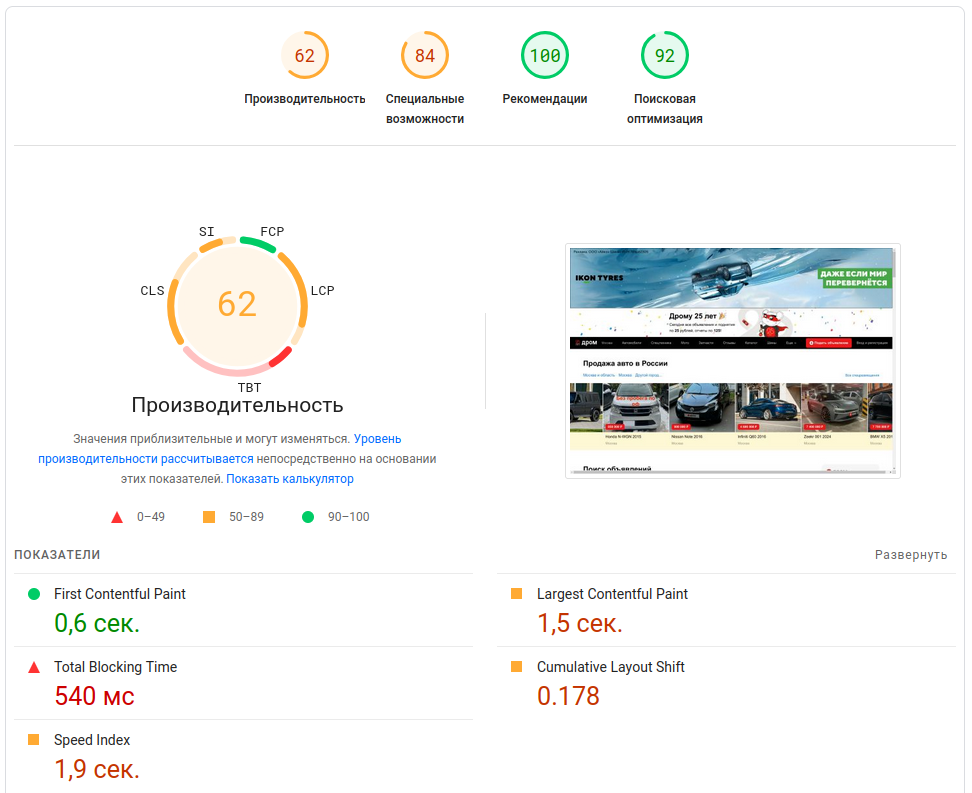
\includegraphics[width=\linewidth]{drom_diag2}}
\end{minipage}
\bigskip

\noindent
\begin{minipage}{\linewidth}
    \fbox{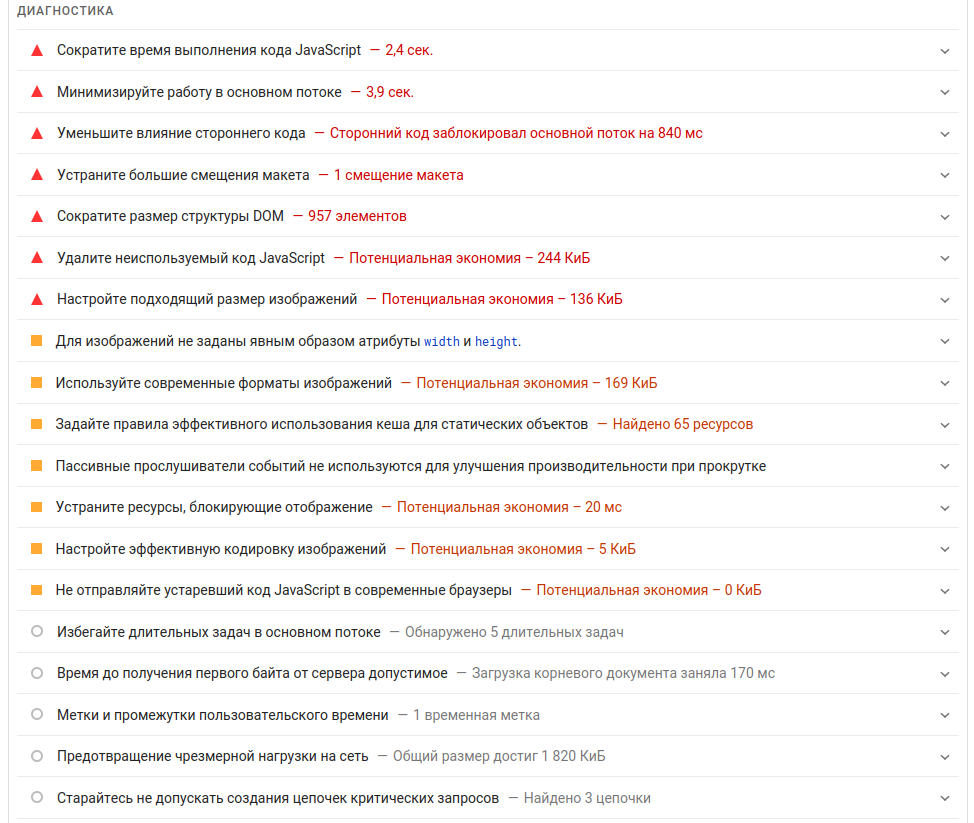
\includegraphics[width=\linewidth]{drom_diag3}}
\end{minipage}
\bigskip

На сайте присутствуют изображения неподходящего размера, в несовременных форматах, в неэффективной кодировке. Суммарная потенциальная экономия - 310 КиБ.

\textbf{sberauto.com}
\bigskip

\noindent
\begin{minipage}{\linewidth}
    \fbox{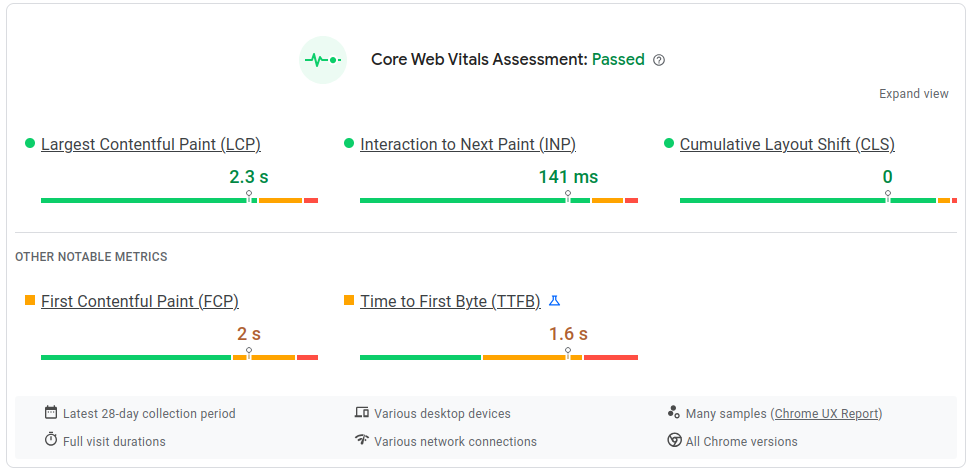
\includegraphics[width=\linewidth]{sberauto_diag1}}
\end{minipage}
\bigskip

\noindent
\begin{minipage}{\linewidth}
    \fbox{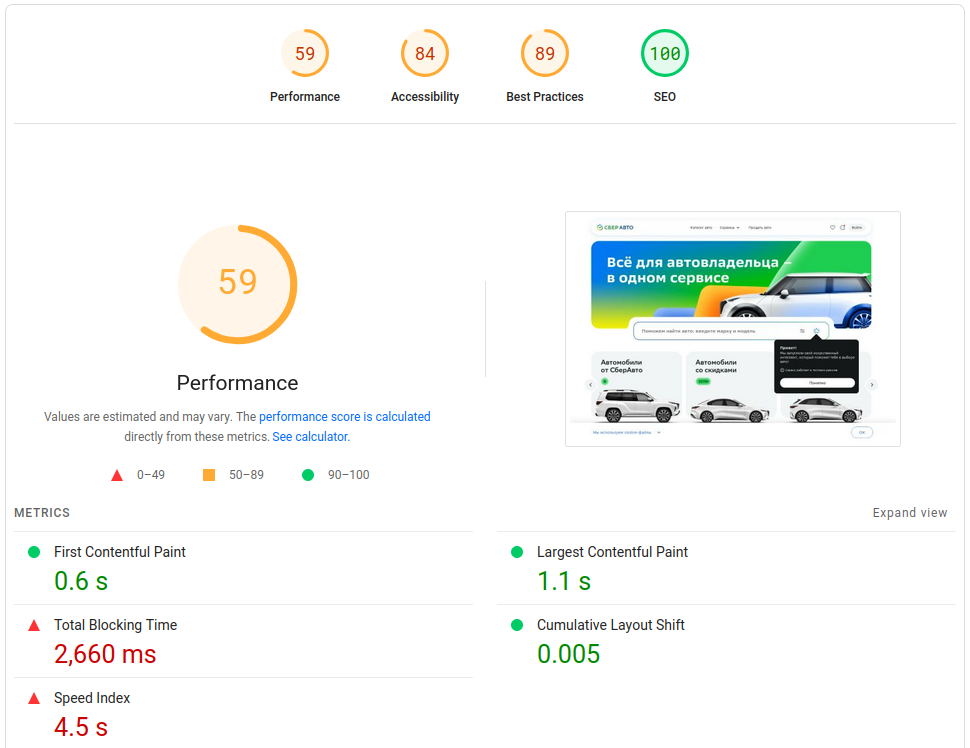
\includegraphics[width=\linewidth]{sberauto_diag2}}
\end{minipage}
\bigskip

\noindent
\begin{minipage}{\linewidth}
    \fbox{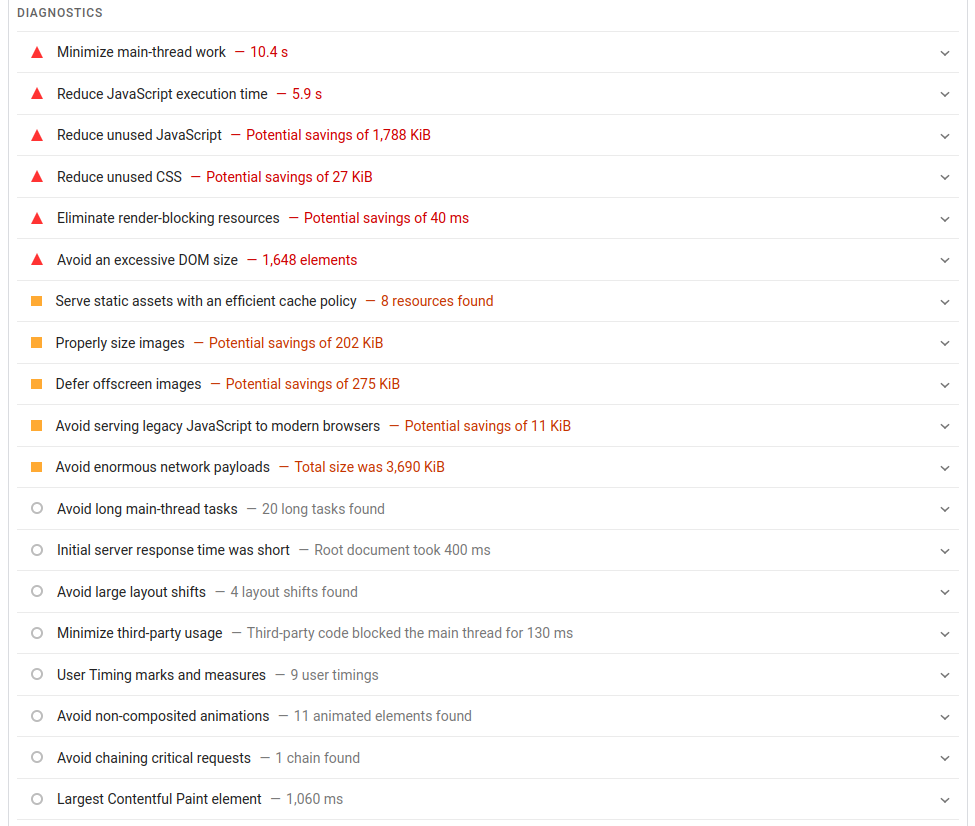
\includegraphics[width=\linewidth]{sberauto_diag3}}
\end{minipage}
\bigskip

На сайте присутствуют изображения неподходящего размера. Суммарная потенциальная экономия - 202 КиБ.

\textbf{mobile.de}
\bigskip

\noindent
\begin{minipage}{\linewidth}
    \fbox{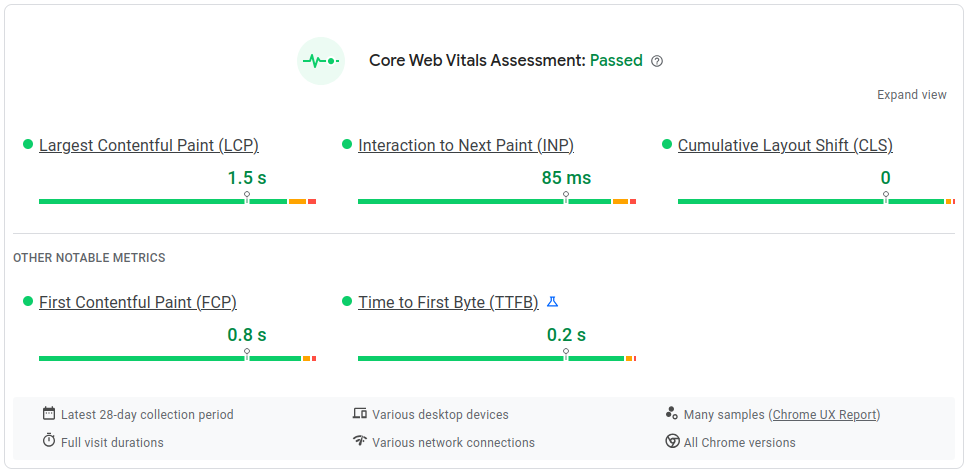
\includegraphics[width=\linewidth]{mobile_diag1}}
\end{minipage}
\bigskip

\noindent
\begin{minipage}{\linewidth}
    \fbox{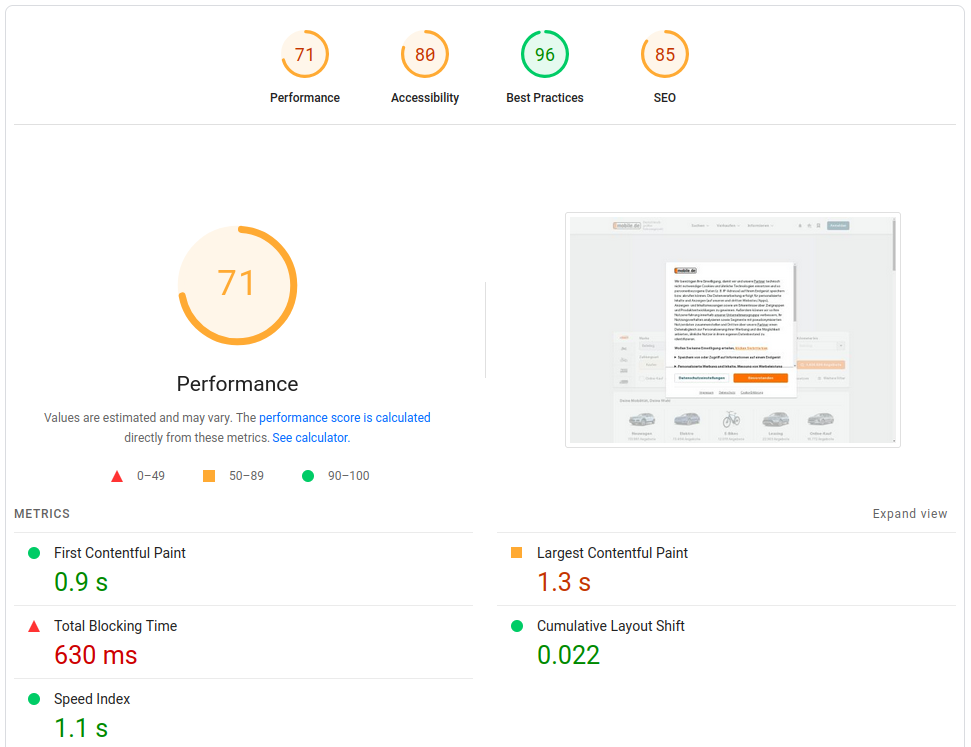
\includegraphics[width=\linewidth]{mobile_diag2}}
\end{minipage}
\bigskip

\noindent
\begin{minipage}{\linewidth}
    \fbox{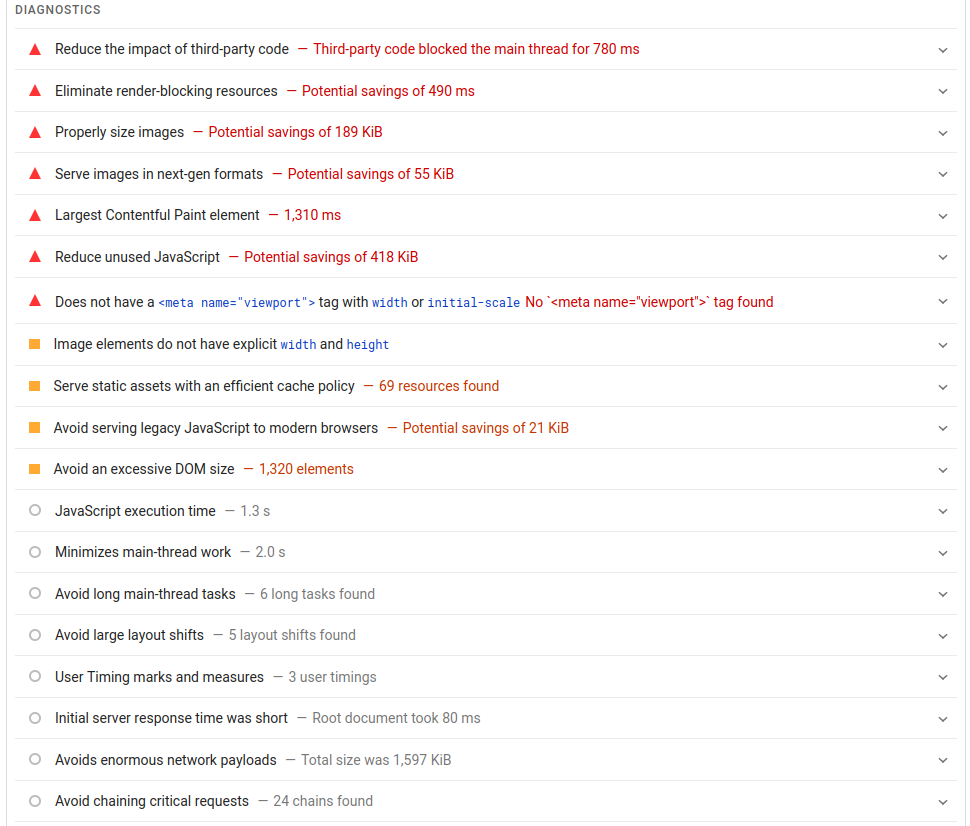
\includegraphics[width=\linewidth]{mobile_diag3}}
\end{minipage}
\bigskip

На сайте присутствуют изображения неподходящего размера, в несовременных форматах. Суммарная потенциальная экономия - 244 КиБ.

\textbf{autoscout24.com}
\bigskip

\noindent
\begin{minipage}{\linewidth}
    \fbox{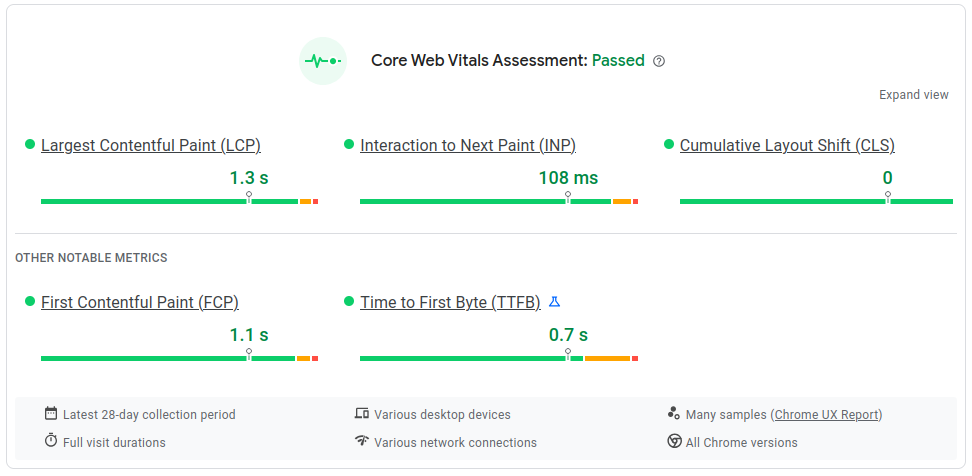
\includegraphics[width=\linewidth]{autoscout24_diag1}}
\end{minipage}
\bigskip

\noindent
\begin{minipage}{\linewidth}
    \fbox{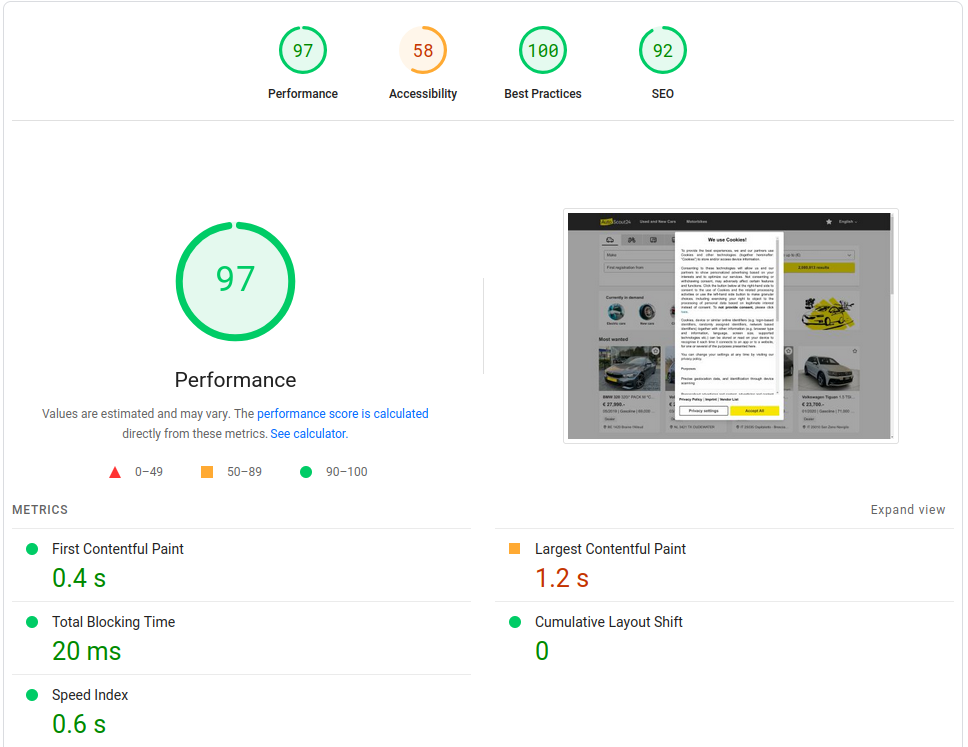
\includegraphics[width=\linewidth]{autoscout24_diag2}}
\end{minipage}
\bigskip

\noindent
\begin{minipage}{\linewidth}
    \fbox{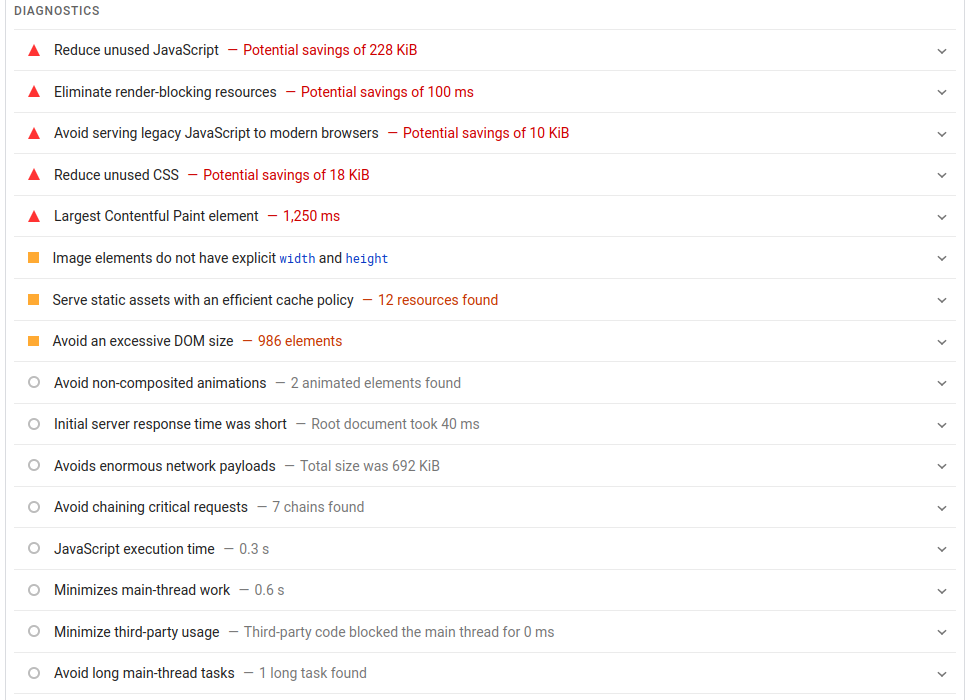
\includegraphics[width=\linewidth]{autoscout24_diag3}}
\end{minipage}
\bigskip

На сайте нет проблем с изображениями.
\bigskip

\textbf{Сводная таблица}

\begin{table}[H]
    \small
\begin{tabular}{|l|l|l|l|l|l|}
\hline
    \textbf{Проблемa} & \textbf{auto.ru} & \textbf{drom.ru} & \textbf{sberauto} & \textbf{mobile.de} & \textbf{autoscout24} \\
\hline
    Неподходящий размер & 23 КиБ & 136 КиБ & 202 КиБ & 189 КиБ & Нет \\
\hline
    Несовременные форматы & 25 КиБ & 169 КиБ & Нет & 55 КиБ & Нет\\
\hline
    Неэффективная кодировкa & Нет & 5 КиБ & Нет & Нет & Нет\\
\hline
\end{tabular}
\end{table}

Учитывая тематику, стиль, палитру, целевую аудиторию были подобраны следующие изображения:

\noindent
\begin{minipage}{\linewidth}
    \fbox{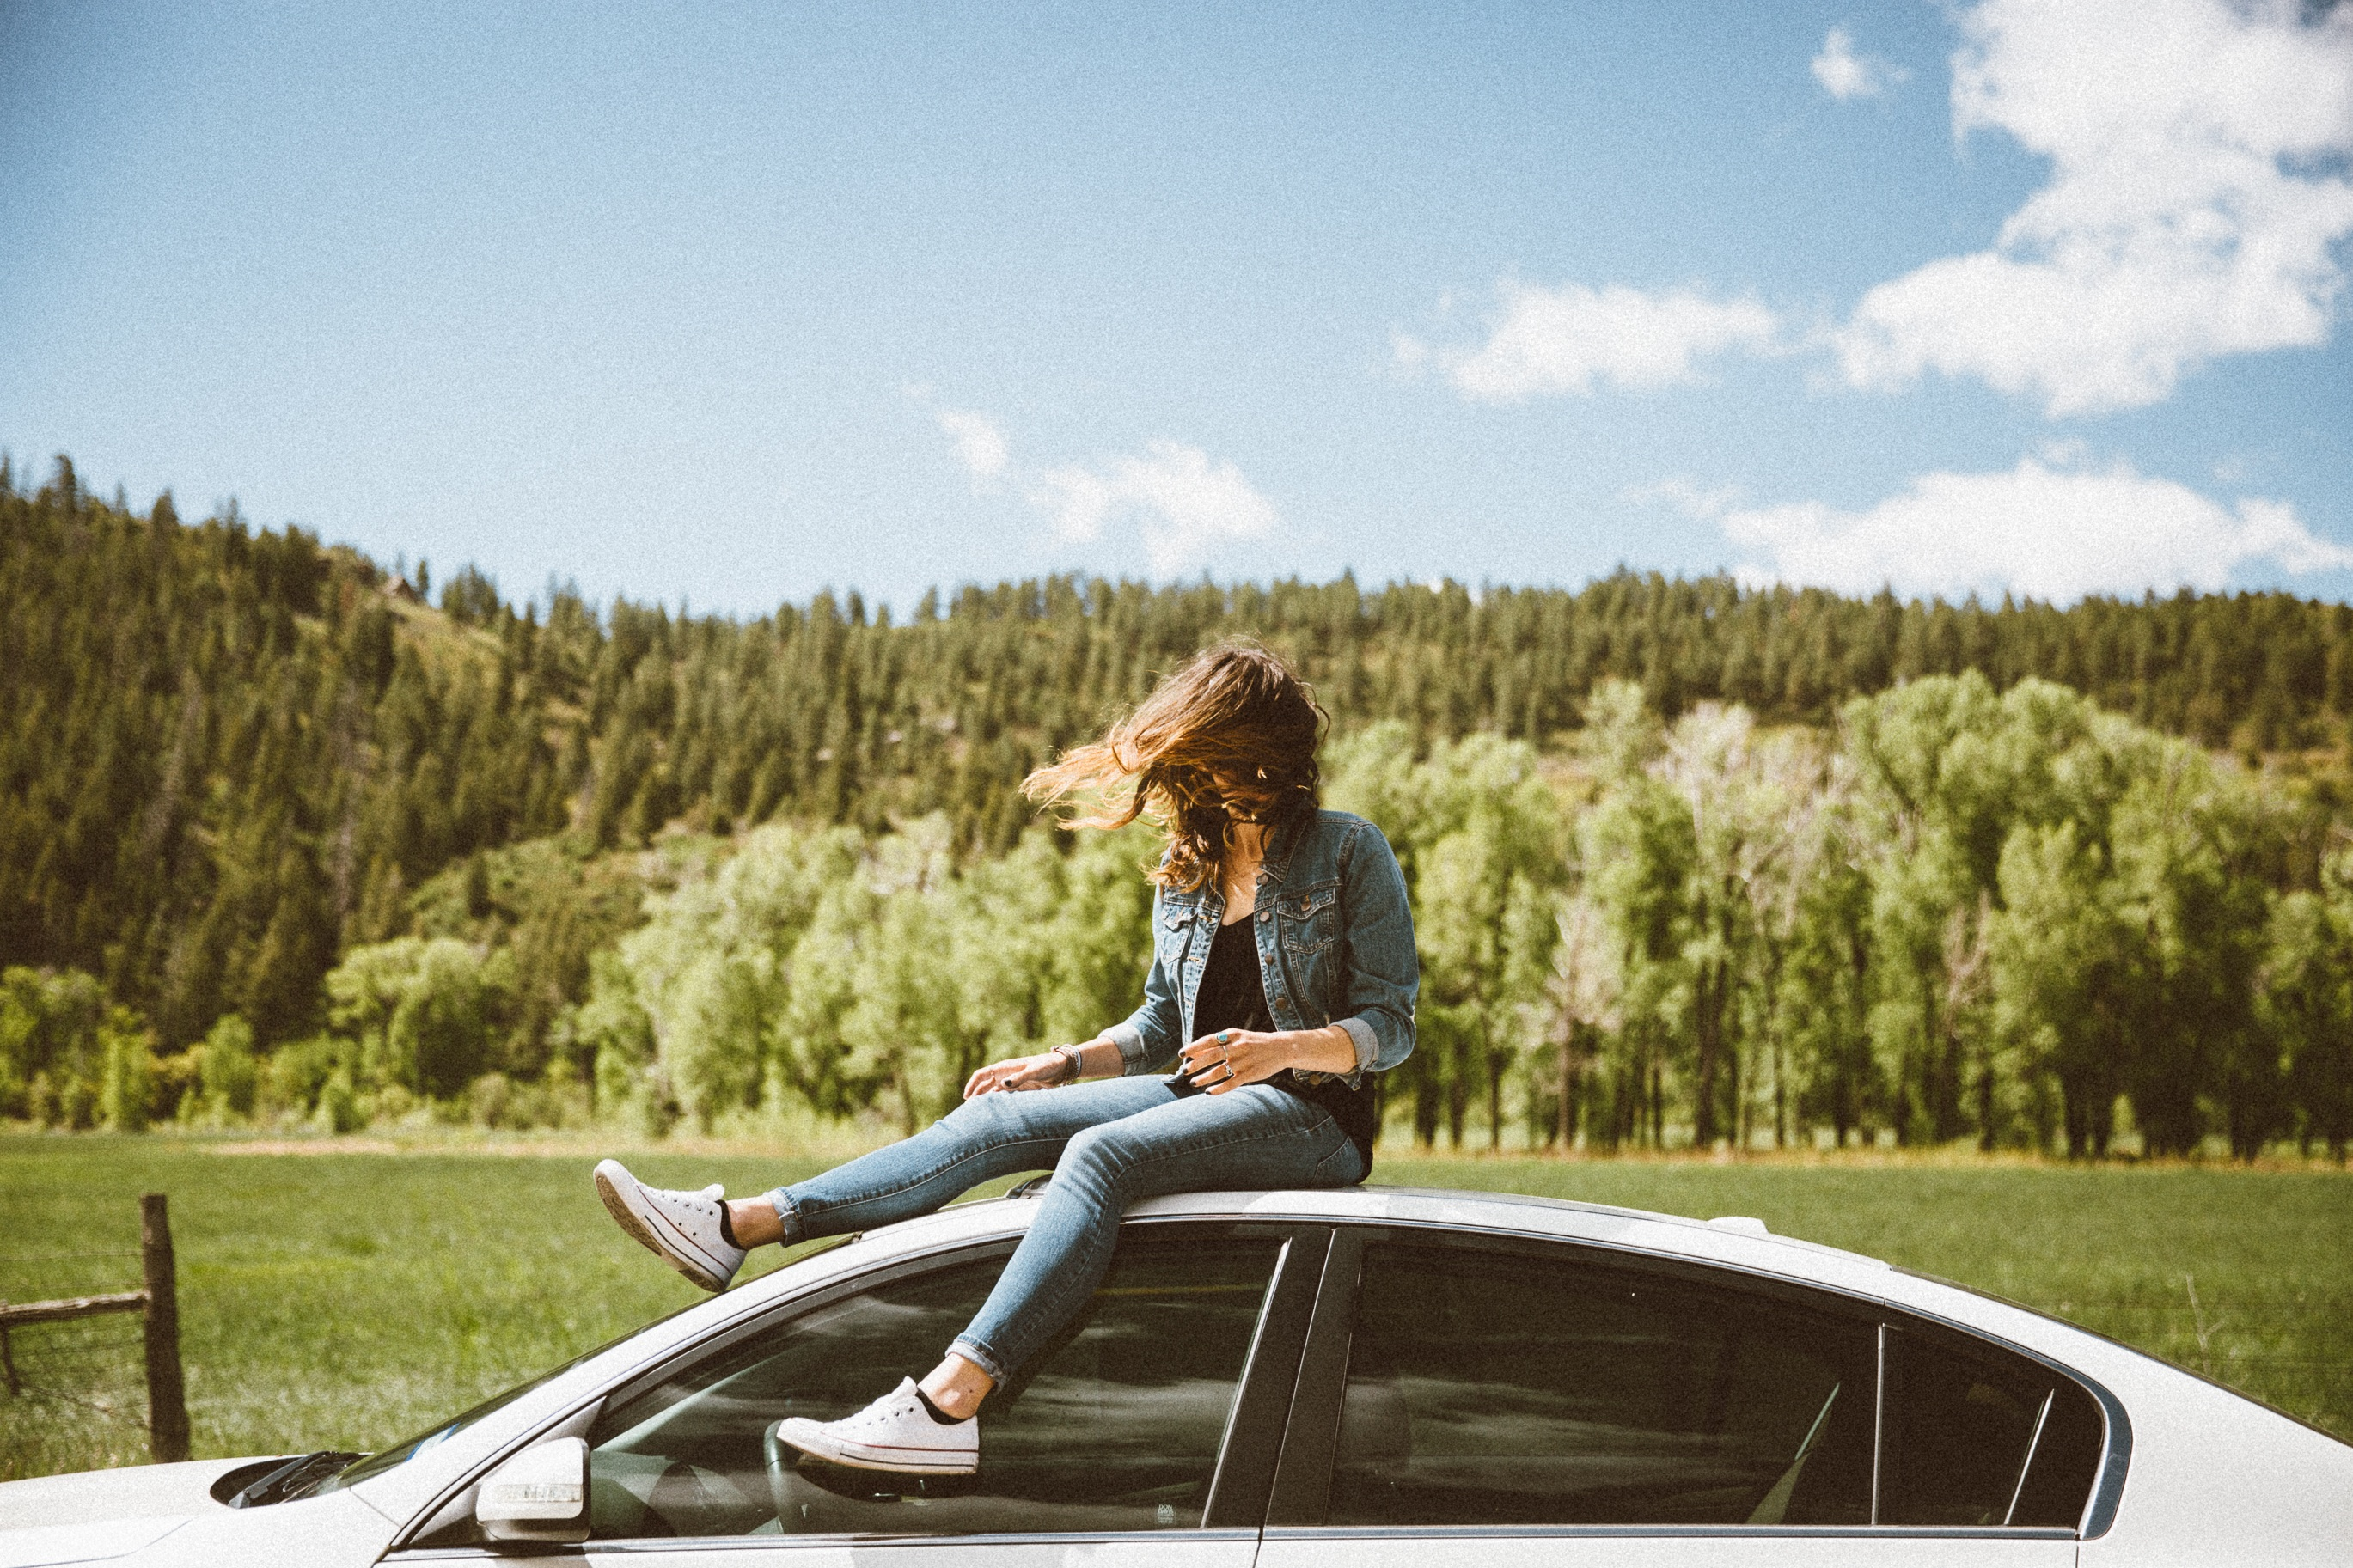
\includegraphics[width=\linewidth]{nature}}
    \captionof{figure}{Источник: icons8.com/photos}
\end{minipage}
\bigskip

\noindent
\begin{minipage}{\linewidth}
    \fbox{\includegraphics[width=\linewidth]{step_mashina_loshadi}}
    \captionof{figure}{Источник: icons8.com/photos}
\end{minipage}
\bigskip

Изображения фотографические, в формате JPG, реализуемы во всех браузерах.

\noindent
\begin{minipage}{\linewidth}
    \fbox{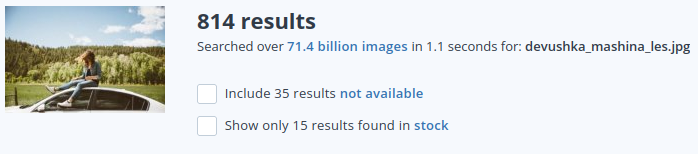
\includegraphics[width=\linewidth]{nature_tineye}}
    \captionof{figure}{Анализ на уникальность через сервис tineye.com}
\end{minipage}
\bigskip

\noindent
\begin{minipage}{\linewidth}
    \fbox{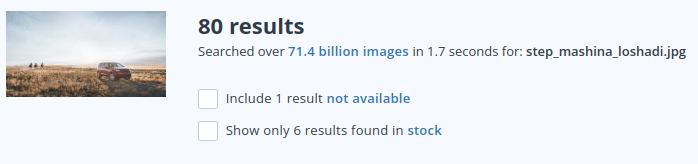
\includegraphics[width=\linewidth]{step_tineye}}
    \captionof{figure}{Анализ на уникальность через сервис tineye.com}
\end{minipage}
\bigskip

\noindent
\begin{minipage}{\linewidth}
    \fbox{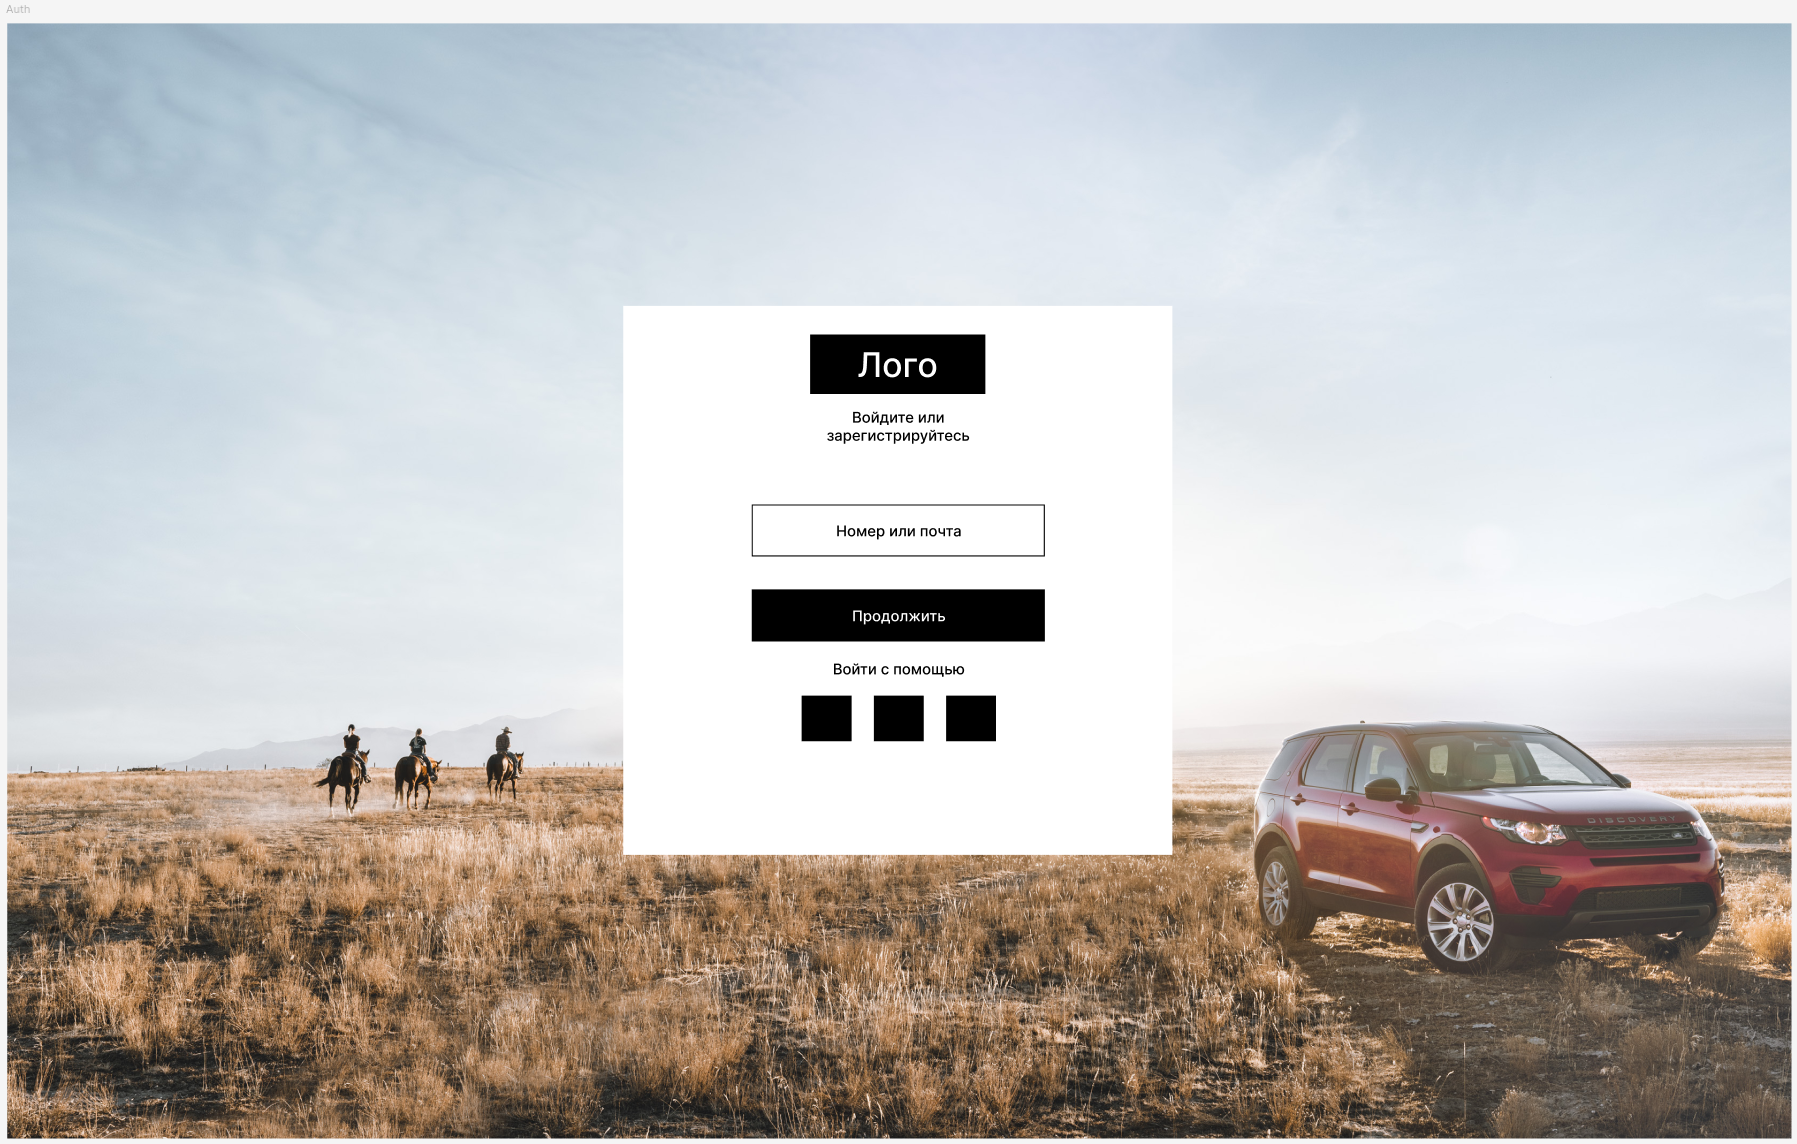
\includegraphics[width=\linewidth]{figma2}}
    \captionof{figure}{Макет}
\end{minipage}
\bigskip

\noindent
\begin{minipage}{\linewidth}
    \fbox{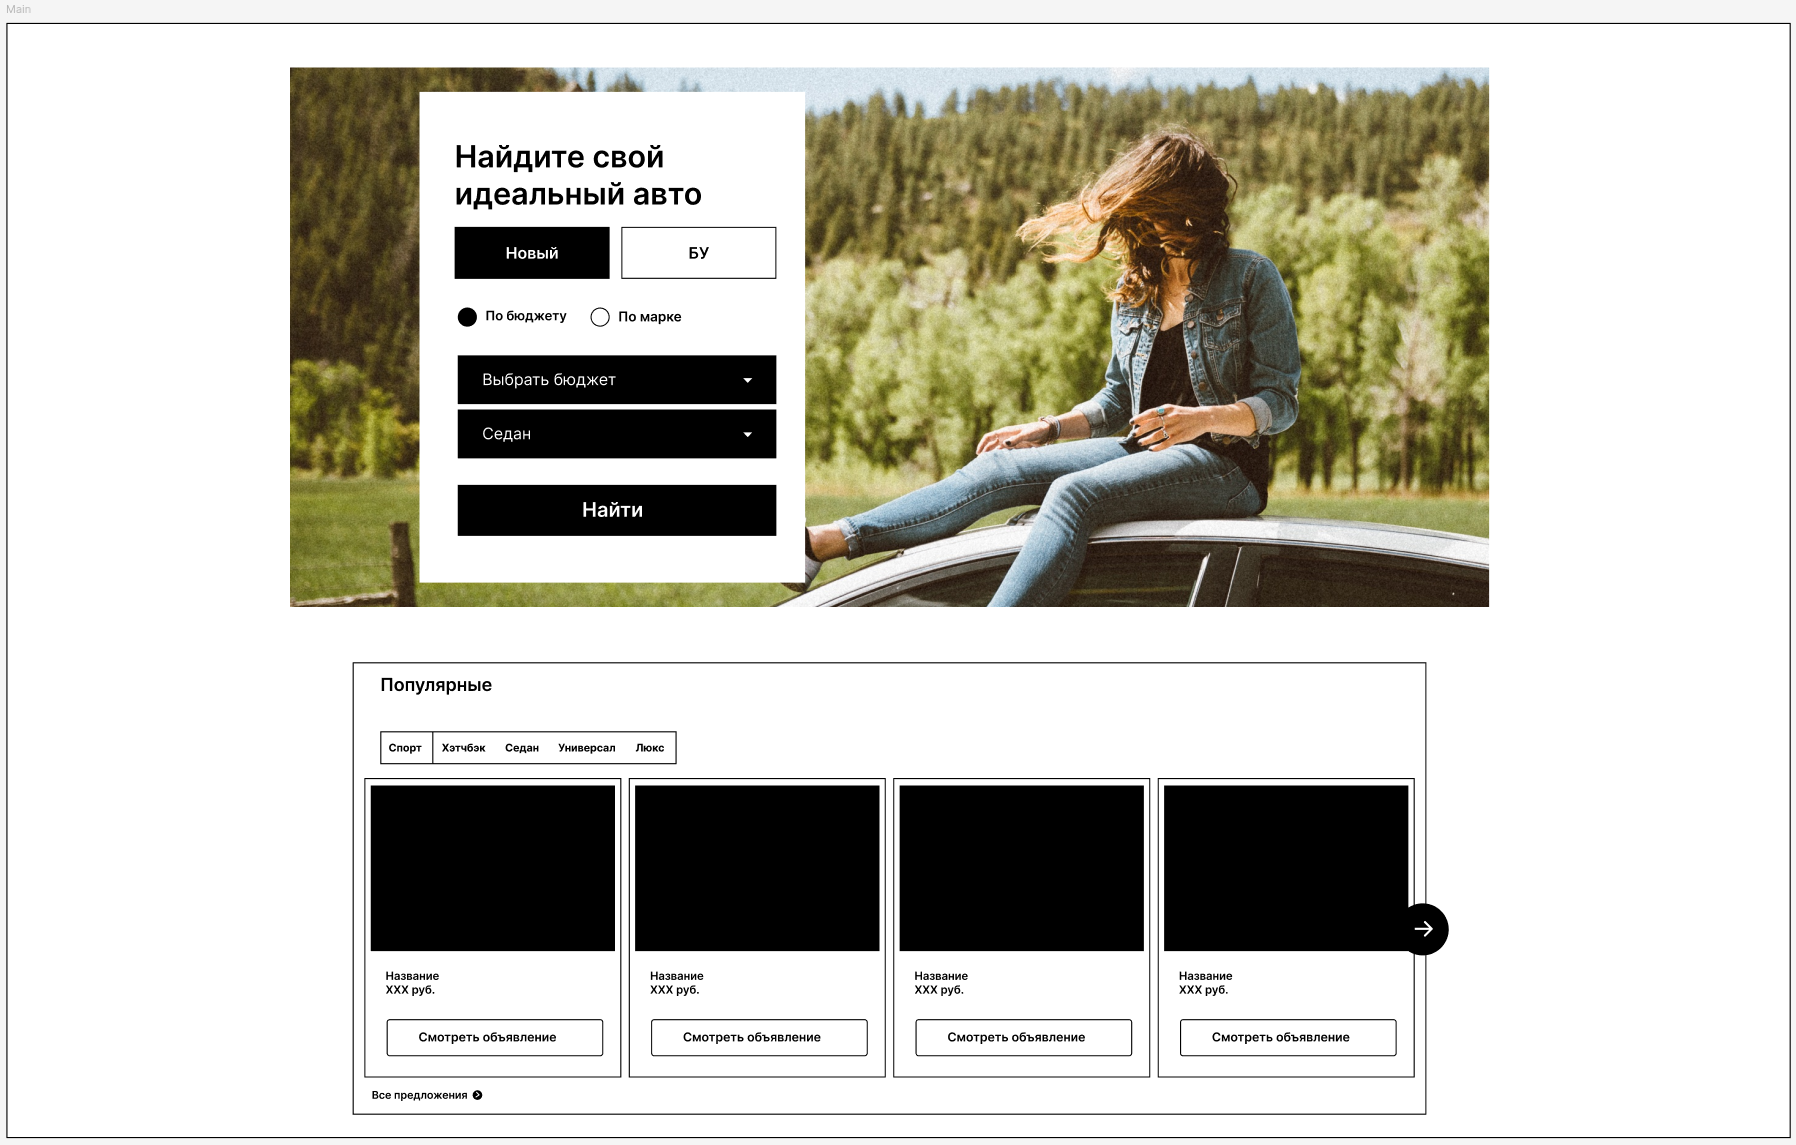
\includegraphics[width=\linewidth]{figma1}}
    \captionof{figure}{Макет}
\end{minipage}
\bigskip

https://www.figma.com/design/25STw8qqDFUKFnCIDQb1ri/Untitled?node-id=54-4&t=OsjLYGum8sn4em53-1

\textbf{Контрольные вопросы и ответы}

\begin{enumerate}
    \item Какими критериями определяется подбор изобразительного контента сайта?Какие виды изобразительной информации используются для веб?

        Соответствие тематике, соответствие аудитории, соответствие стилю и палитре, соответствие высокому качеству, уникальность, эмоциональная привлекательность.
        \bigskip

        Виды изобразительной информации:
        фотографии, иллюстрации, логотипы, иконки, 3D графика.
    \item Какую роль играют параметры изображений для веб?

        Размер изображения влияют на скорость загрузки страницы, разрешение влияет на четкость изображения, формат влияет на качество и размер файла.
    \item На что необходимо опираться при выборе фотографических изображений

        На качество изображения, соответствие тематике, стиль должен соответствовать остальным элементам дизайна.
    \item Какие существуют рекомендации разрешению и «весу» изображений для веб интерфейса?

        Использовать разрешение не более 1024 пикселей в ширину (кроме фоновых изображений), размер сохранять в пределах 80-100 килобайт, использовать форматы: JPEG, PNG, WebP, AVIF, GIF, SVG.
    \item Какие существуют приемы по подготовке изображений для веб-интерфейса?

        Сжатие изображения без потери качества, подгонка под необходимые размеры, заполнение alt-атрибутов, выбор правильно формата.
\end{enumerate}

\end{document}
